\section{ADMM Hardware Architecture}\label{arch}
This section introduces the detailed hardware architecture to support Algorithm\cref{alg:ADMM}. Major focuses of the design were system parametrization, system scaling, and runtime reference trajectory setting. Finally, we analyze the computation latency and BRAM usage. The design is written in VHDL using Vivado 2015.4 IDE.
\subsection{ADMM Architecture Overview}
As shown in Fig.\cref{fig_arch}, the high-level hardware architecture is divided into Top and Bottom level for a modularized illustration. Top level is the Quadratic Programming Solver. It has a matrix-vector multiplier tree structure. Bottom level is composed of three parts: 1) Saturation Function (marked in green diagonal line), 2) Update Vector $\upsilon^i$ (marked in purple cross line), 3) Update Vector $l$ (marked in red). Some FIFOs which are used to store intermediate values are not shown in the figure. We use Block RAM(BRAM) to store the $\zeta^i$, $\upsilon^i$ vector and the boundary value box constraints $x$, $u$, and $\Delta u$.

\begin{figure}[t]
\centering
\captionsetup{justification=centering}
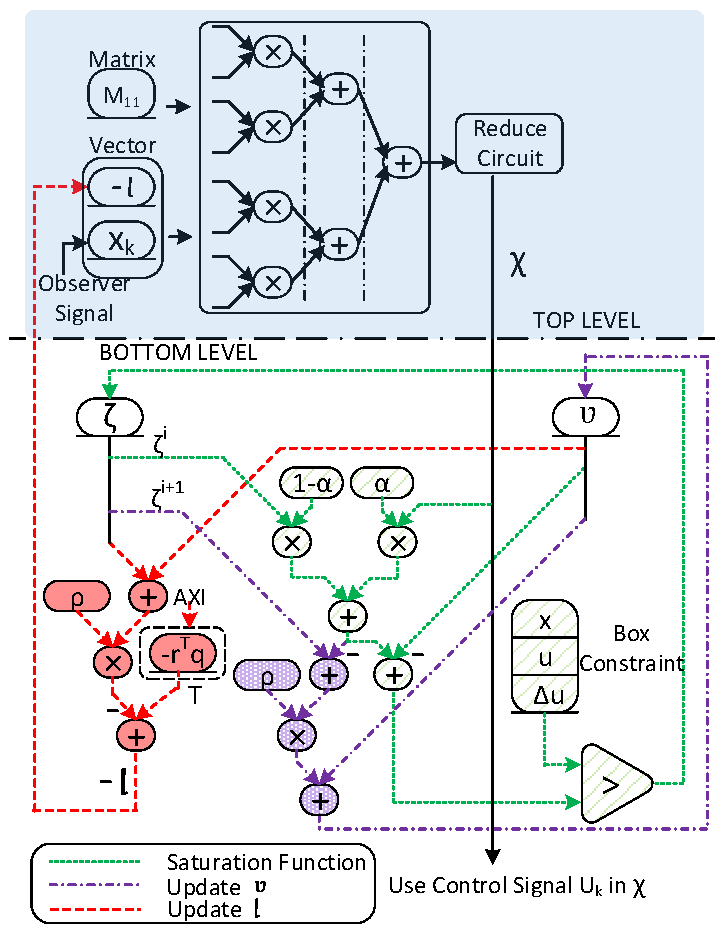
\includegraphics[scale=.59]{../figure/architecture.pdf}
\DeclareGraphicsExtensions.
\caption{Hardware Architecture for ADMM with Relaxation Parameter $\alpha$.\label{fig_arch}}
\end{figure}

We next describe the components of Fig.\cref{fig_arch} in greater detail:
\subsubsection{Matrix-vector Multiplier (MVM)}
The QP solver is similar to the architecture presented in\cite{Zhuo:2005:SMM:1046192.1046202} for parallelizing MVM of large sparse matrices. The MVM computation uses a tree structure. $D_p$ indicates the depth of the MVM tree. The total number of multipliers in the MVM tree is $2^{D_p}$ and the number of adders is $2^{D_p}-1$.

\subsubsection{Data Storage}
Block RAMs (BRAMs) are used as the primary on-chip memory of the MPC engine. We configure the BRAMs as true dual port, which provides two read and two write ports. Every multiplier in the MVM tree has a dedicated dual port BRAM attached, with one port feeding matrix data and one port feeding vector data.\par

According to the BRAM configuration datasheet, the BRAM has to be at least 36Kb. Since the matrix size is the square of the vector size, we reserve a small fraction of space for vector storage. Another solution is to use Look Up Tables (LUTs) to store the vector. In either case, the vector should be duplicated to avoid write back conflicts.\par
%18 Kb BRAM alone cannot be configured as true dual port BRAM. Thus each multiplier has to be attached with at least one 36 Kb BRAM, where only 32Kb memory is available when the data width is set as 32 bit. The system cascades 18Kb BRAM with the 36Kb BRAM to expand its storage. The number of 18Kb BRAM required for each multiplier is $\lceil max(N_E,1024)/512\rceil$. As we mentioned, $N_E$ is the number of matrix element we stored in the BRAM. The percentage of BRAM utilization in front of each multiplier is shown in Equation\cref{eq:uti}. Fig.\cref{fig_bram3} shows the BRAM unilization, which varies with $N_E$ in that BRAM. With this figure, we can easily know the utilization of BRAMs after we compute the number of matrix element inside. Generally with more and more matrix data stored in the BRAM, the utilization will increase.
%
%\begin{equation}
%\label{eq:uti}
%Utilization=\frac{N_E}{\lceil \frac{max(N_E,1024)}{512}\rceil *512}
%\end{equation}
%
%\begin{figure}[!ht]
%\centering
%\captionsetup{justification=centering}
%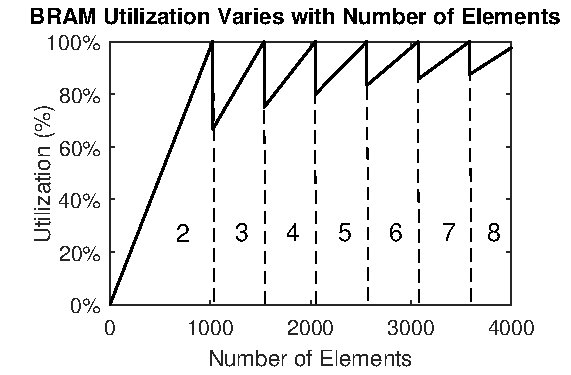
\includegraphics[scale=.78]{../figure/BRAM3.pdf}
%\DeclareGraphicsExtensions.
%\caption{The utilization of BRAMs varies with number of elements stored regarding each multiplier. The digital number between dash line and solid line is the number of 18Kb BRAM attached in front of each multiplier.\label{fig_bram3}}
%\end{figure}

We use $N_{BRAM}$ to represent the number of available 36Kb BRAMs. $N_{DSP}$ is the number of DSP slices on-chip. If the hardware resources meet inequality condition\cref{eq:com}, the BRAM will hinder the scalability of the system without the support of the reduce circuit. This conclusion is based on the assumptions that 1) each multiplier and adder consume one DSP slice; 2) each MVM multiplier requires at least one 36kb BRAM.
According to the Zynq datasheet, only the Z-7100 device from the Zynq-7000 family is unconformable to the inequality condition\cref{eq:com}, which indicates that the on-chip memory is the resource bottleneck for most of the Zynq-7000 family.
\begin{equation}
\label{eq:com}
2*N_{BRAM}\geq N_{DSP}\geq 63.25\sqrt{N_{BRAM}}
\end{equation}

%\subsection{Potential Computation Parallism Estimation}
%\label{aaa}
%The computation can be further paralleled by introducing multiple processing units (PUs) as is shown in Fig.\cref{fig_hp}. Each PU has its own ADMM component like in Fig.\cref{fig_arch}. 
%The $M_{11}$ matrix is separated row by row. We store each row from PU\big[1\big] to PU\big[K\big] and start over until the whole matrix is stored into PU BRAMs. In this way, we can avoid conflict of writing vector back if their destination is the same BRAM. After the data fills the processing pipeline, $K$ new vector elements will come out of the pipeline during the same clock cycle. Since these elements are stored in different BRAMs, the write-back operation can be done in one clock cycle. We call this mechanism duplication.
%
%\begin{figure}[!ht]
%\centering
%\captionsetup{justification=centering}
%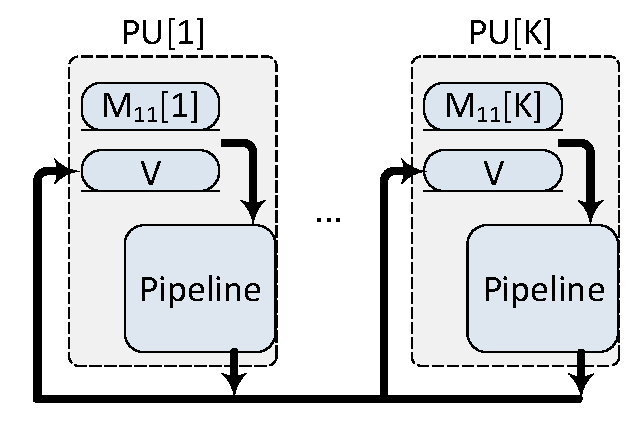
\includegraphics[scale=.40]{../figure/highParallel.pdf}
%\DeclareGraphicsExtensions.
%\caption{Highly paralleled ADMM Hardware Solution\label{fig_hp}}
%\end{figure}
%
%The latency shares the same formula as Equation.\cref{eq:tl} except for the $L_{read\_ M_{11}}$ term. The $L_{read\_ M_{11}}$ is inverse proportional to parallelism $K$ in Equation.\cref{eq:klemr} .
%\begin{equation}
%\label{eq:klemr}
%L_{read\_ M_{11}}=\frac{N_{ROW}}{K}*(N_R+1)
%\end{equation}

\subsubsection{Reduce Circuit}

The purpose of the reduce circuit is to let us balance between resource usage and the number of MVM pipeline stages. Fig.\cref{fig_red} shows a reduce circuit structure, which is cascading two smaller reduce circuits.\par
\begin{figure}[t]
\centering
\captionsetup{justification=centering}
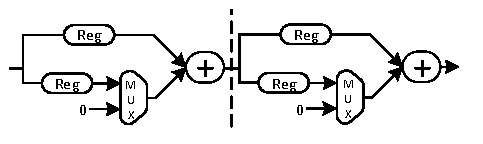
\includegraphics[scale=0.9]{../figure/Reduce.pdf}
\DeclareGraphicsExtensions.
\caption{Reduce Circuit Architecture with Two Cascaded Adders\label{fig_red}}
\end{figure}
The reduce circuit allows a single row of the matrix and vector to be separated into segments, and each segment is fed into the MVM pipeline in consecutive clock cycles. The reduce circuit accumulates the sum of each segment and generates a final result out of the last reduce stage. By employing more cascading levels, we can divide each row of the matrix into smaller segments at the cost of increasing latency due to increased pipeline stages at the reduce circuit. Suppose the depth of the MVM tree is $D_p$, and the number of $M_{11}$ rows is $N_{ROW}$ and columns is $N_{COL}$. Then the number of adders in the reduce circuit that our system requires is $N_R=\lceil N_{COL}/2^{D_p}\rceil-1$. The number of clock cycles to merge all the matrix and vector data into the MVM pipeline is:
\begin{equation}
\label{eq:md}
L_{read\_ M_{11}}=N_{ROW}*(N_R+1)
\end{equation}

\subsubsection{Saturation Function}
Fig.\cref{fig_arch} contains the hardware for saturation function. We assume each variable has same absolute upper and lower boundary value so that we just store the positive boundary values in the box constraint BRAM. The result of $\chi^{i+1}-\upsilon^{i}$ is compared with the box constraints. If the absolute value of $\chi^{i+1}-\upsilon^{i}$ is smaller than the box constraint, we output the value directly. Else, if the value is larger, we output the box constraint using the sign of $\chi^{i+1}-\upsilon^{i}$.

\subsection{Trajectory Setting During Runtime}
\begin{figure}[t]
\centering
\captionsetup{justification=centering}
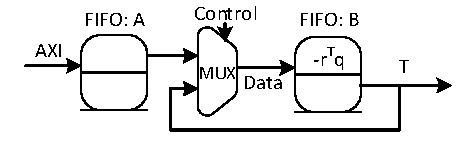
\includegraphics[scale=.75]{../figure/trajectoryProfile.pdf}
\DeclareGraphicsExtensions.
\caption{Runtime Trajectory Planning\label{fig_traj}}
\end{figure}

MPC can optimize a system's following of a trajectory multiple time steps ahead so that system can react accordingly in advance. Our controller can set the desired trajectory during runtime. For example, we may want to update a UAV's flight path while it is in the air.\par

We use two FIFOs to realize the functionality. The architecture is shown in Fig.\cref{fig_traj}, which is located in the dashed square marked by 'T' in Fig.\cref{fig_arch}. First, we configure FIFO:A and FIFO:B. FIFO:B stores the trajectory data for the current computation, and FIFO:A stores the future trajectory data. When computing the $l$ vector, we read FIFO:B, use the data and write its output back to itself, which will be used for next converge iteration. In the last iteration, we discard the front $N$ numbers after reading, and write the remaining back to FIFO:B. Next, we load $N$ new trajectory data from FIFO:A into FIFO:B. In this way, each trajectory data shifts forward one sample step, and we fill the last trajectory point with a new one. Since writing to FIFO:A is independent of operations on FIFO:B, we can write new state trajectory data to FIFO:A at any time before FIFO:B goes empty.

\subsection{Latency Analysis}

Table\cref{tab:lat} gives computation latency. The floating point multiplier latency is $L_M$=8; the floating point adder latency is $L_A$=11, the comparator latency is $L_C$=2. We call $L_{bt}+L_{bl}$ pure processing stages, namely the number of pipeline stages from an element entering the MVM pipeline to finishing.

\begin{center}
\captionof{table}{Computation Latency}
\label{tab:lat}
\begin{tabular}{ c|c } 
 \hline
 Binary Tree ($L_{bt}$)& $L_M+D_pL_A+N_R(L_A+2)$\\ 
\hline
 Bottom Level ($L_{bl}$)& $6L_A+3L_M+L_C$\\ 
 \hline
\end{tabular}
\end{center}

%To be noticed here, the result can only be written back into BRAM after all the matrix and vector data have been merged into the MVM pipeline since the two ports of each BRAM are being used as reading ports (one for the matrix $M_{11}$, one for the vector $V$) during the time. Assuming the data is blocked for $L_f$ pipeline stages in the form of walking through the FIFO in the lower-left portion of Fig.\cref{fig_arch} before writing back, then $L_f$ is computed as in Equation\cref{eq:lf}. 
%\begin{equation}
%\label{eq:lf}
%L_{f}=max\Big(0,L_{mer}-(L_{bt}+L_{bl})\Big)
%\end{equation}
%
%The total clock cycle for doing one iteration of Algorithm\cref{alg:ADMM} is:
%\begin{align*}
%L_{ADMM}&=L_f+L_{bt}+L_{bl}+L_{mer}\\
%&=max\Big(2*L_{mer},L_{mer}+L_{bt}+L_{bl}\Big)
%\numberthis \label{eq:tl}
%\end{align*}
%
%From Formula\cref{eq:tl} we see that if $L_{mer}$ is greater than $L_{bt}+L_{bl}$, the total pipeline stages is irrelative to the pure processing stages. This finding means that even though fixed-point adder/multiplier takes one single clock cycle to get to the result, for a large matrix, the pipeline stages in Figure.\cref{fig_arch} has no effect on your total processing time $L_{ADMM}$, which proves that floating-point is as fast as fixed-point arithmetic in this situation. 

The total latency $L_{ADMM}$ is shown in Equation.\cref{eq:tl}, which is the sum of pure processing stages and the clock cycles to finish fetching all the matrix and vector data into MVM tree ($L_{read\_ M_{11}}$). 
\begin{equation}
\label{eq:tl}
L_{ADMM}=L_{bt}+L_{bl}+L_{read\_ M_{11}}
\end{equation}

The architecture by default fetches one row per clock cycle or we can break each row into several pieces and accumulate each piece through the reduce circuit. However, under most cases, $N_{COL}/2^{D_p}$ is not an integer, thus some BRAMs store '0's to pad the final piece of the matrix row. These padding '0's occupy BRAM space and decrease the scalability of the design. The problem can be solved via introducing a simple state machine that tells the hardware which DSP should be fed '0' instead of reading data from BRAM.

%\subsection{Potential Computation Parallism Estimation}
%\label{PCPE}
%The computation can be further paralleled by introducing multiple processing units (PUs) as is shown in Fig.\cref{fig_hp}. Each PU has its own ADMM component like in Fig.\cref{fig_arch}. 
%%The reduce circuit is no more recommended in this scenario since the on-chip resource is not considered as a limitation. 
%The $M_{11}$ matrix is separated row by row. We store each row from PU\big[1\big] to PU\big[K\big] and start over until the whole matrix is stored into PU BRAMs. In this way, we can avoid conflict of writing vector back if their destination is the same BRAM. After the data fills the processing pipeline, $K$ new vector elements will come out of the pipeline during the same clock cycle. Since these elements are stored in different BRAMs, the write-back operation can be done in one clock cycle. We call this mechanism duplication.
%
%\begin{figure}[!ht]
%\centering
%\captionsetup{justification=centering}
%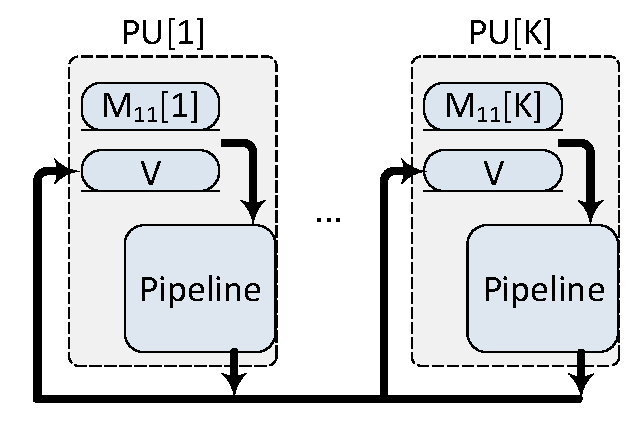
\includegraphics[scale=.55]{../figure/highParallel.pdf}
%\DeclareGraphicsExtensions.
%\caption{Highly paralleled ADMM Hardware Solution\label{fig_hp}}
%\end{figure}
%
%The latency shares the same formula as Equation.\cref{eq:tl} except for the $L_{read\_ M_{11}}$ term. The $L_{read\_ M_{11}}$ is inverse proportional to parallelism $K$ in Equation.\cref{eq:klemr} .
%\begin{equation}
%\label{eq:klemr}
%L_{read\_ M_{11}}=\frac{N_{ROW}}{K}*(N_R+1)
%\end{equation}

